% Chapter Template

\chapter{Ensayos y resultados} % Main chapter title

En este capítulo se menciona los ensayos realizados asi como 

\label{Chapter4} % Change X to a consecutive number; for referencing this chapter elsewhere, use \ref{ChapterX}

%----------------------------------------------------------------------------------------
%	SECTION 1
%----------------------------------------------------------------------------------------

\section{Generación del sistema de pruebas}
\label{sec:pruebasHW}

La idea de esta sección es explicar cómo se hicieron los ensayos, qué resultados se obtuvieron y analizarlos.
\section{Pruebas unitarias}
\subsection{Pruebas del servidor Mosquitto}
Para simular mensajes y observar el comportamiento de cada una de las partes del sistema se utilizó la herramienta MQTT explorer   \citep{WEBSITE:29}.

\begin{figure}[ht]
	\centering
	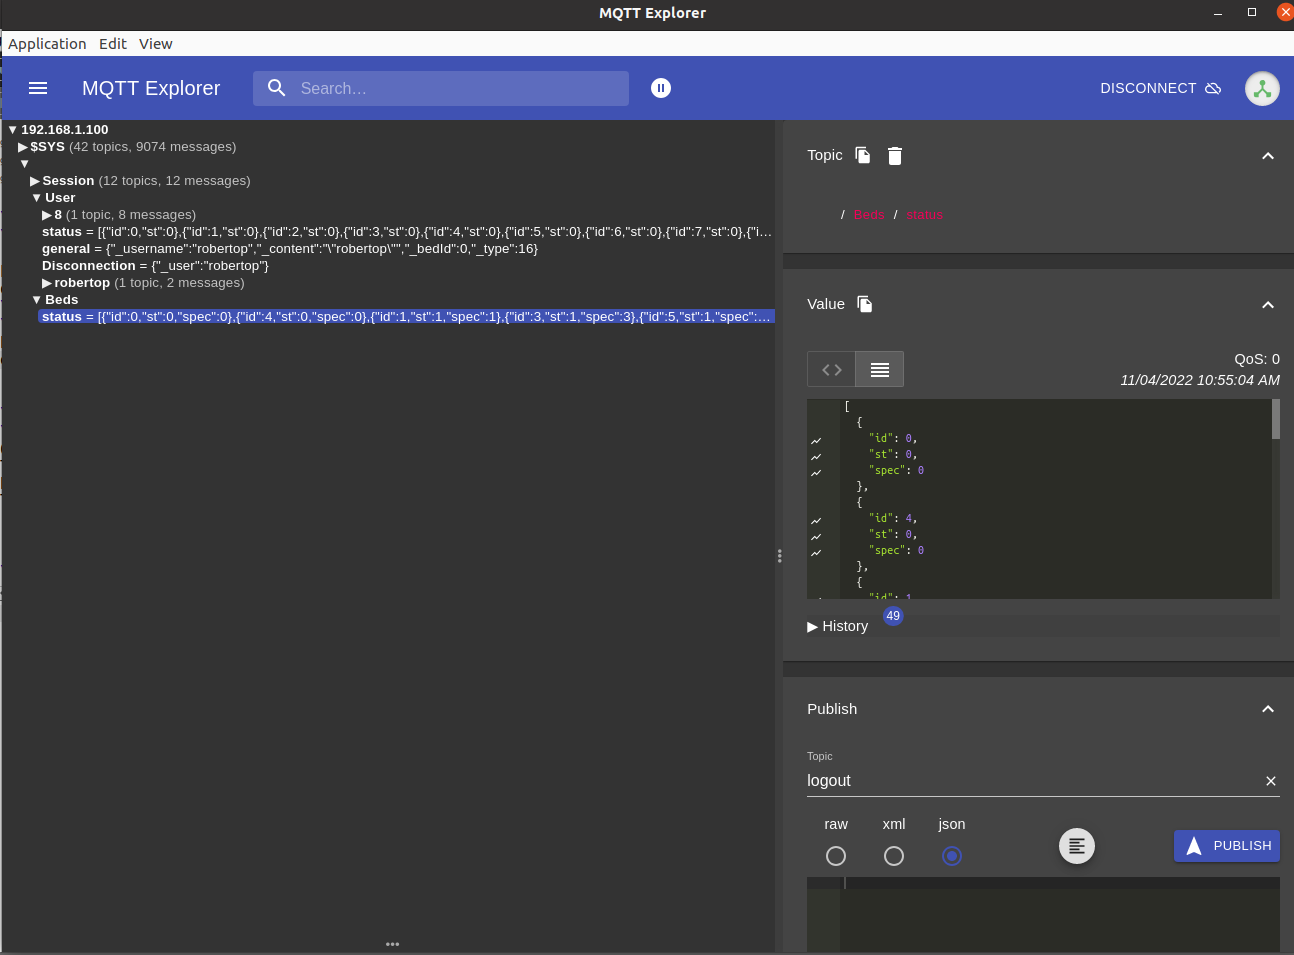
\includegraphics[scale=.25]{./Figures/mqtt-explorer.png}
	\caption{Imagen de MQTT Explorer.}
	\label{fig:MQTT Explorer}
\end{figure}

Esta herramienta fue no solo muy útil para realizar ensayos sino tambien para realizar el desarrollo de las funcionalidades propiamente dichas.

\subsection{Pruebas unitarias de la API Rest}

Para simular el logeo y la consulta a la base de datos se utilizó la herramienta PostMan \citep{WEBSITE:30} y la consola de administrador de phpMyAdmin mencionada en \ref{Chapter2}. En la \ref{fig:Logueo en el sistema con Postman} se observa el \textit{token} devuelto por el backend al logearse con las credenciales correspondientes y en \ref{fig:Rechazo Logueo en el sistema con Postman} se observa la respuesta al ingresar una contraseña inadecuada.

\begin{figure}[ht]
	\centering
	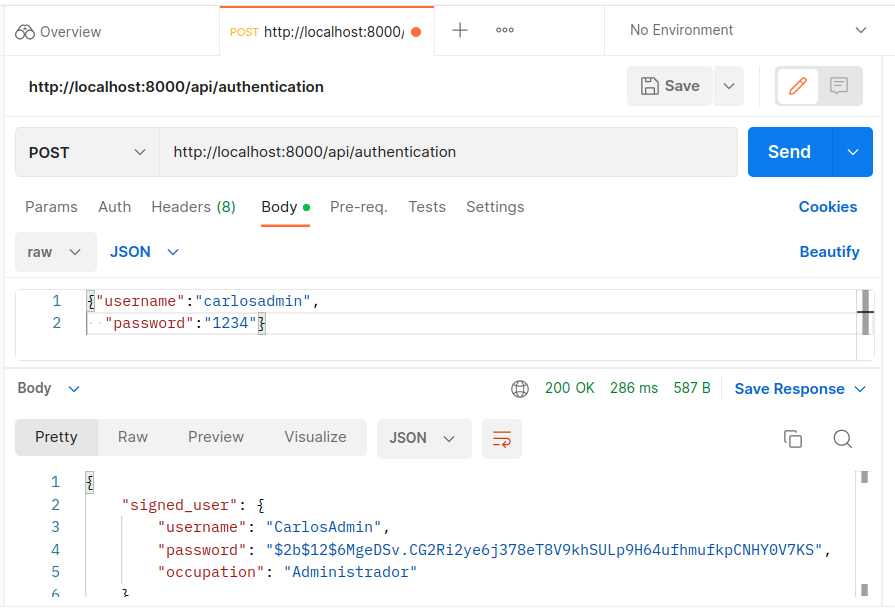
\includegraphics[scale=.35]{./Figures/auth.png}
	\caption{Logueo en el sistema con Postman.}
	\label{fig:Logueo en el sistema con Postman}
\end{figure}

\begin{figure}[ht]
	\centering
	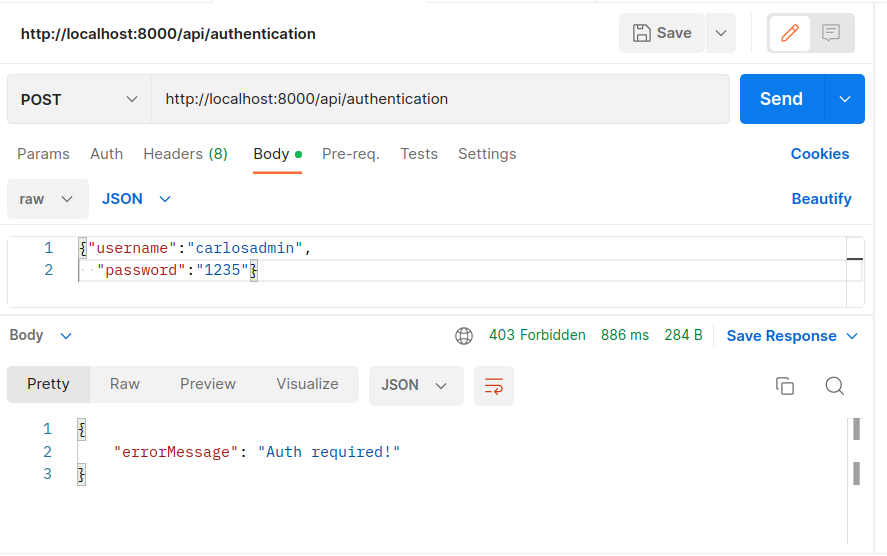
\includegraphics[scale=.35]{./Figures/no-auth.png}
	\caption{Rechazo de logueo.}
	\label{fig:Rechazo Logueo en el sistema con Postman}
\end{figure}


Durante el desarrollo, se deshabilitó la opción de logueo para facilitar las pruebas. 

\section{Integración del sistema}
\subsection{Instalación del sistema en una instancia de AWS}
Con el objetivo de no incorporar costos en las pruebas, se generó una instancia Free Tier en Amazon Web Services, en la cual se instaló Ubuntu, el broker Mosquitto, el backend, la página Web y un servidor NGINX para que funcione como proxy inverso. Tambien se contrató el servicio route 53 que permite customizar las politicas de ruteo.
De esta manera, se puede acceder al sistema desde cualquier dispositivo móvil conectado a una red.

\subsection{Generación/instalación de la aplicación móvil}

\subsection{Equipo simulador de llamadores}

\subsection{Resultados de utilizar el sistema}